% Gemini theme
% See: https://rev.cs.uchicago.edu/k4rtik/gemini-uccs
% A fork of https://github.com/anishathalye/gemini
% Adapted by Nisansa de Silva 27/03/2025

\documentclass[portrait,paperwidth=65cm,paperheight=130cm,fontscale=0.35,dvipsnames]{poster/baposter}

% ====================
% Packages
% ====================
%  width=233.68,height=116.84,
\usepackage[T1]{fontenc}
\usepackage{lmodern}


\usepackage{graphicx}
\usepackage{caption}
\usepackage{booktabs}
\usepackage{hhline}
\usepackage{tikz}


\definecolor{maroon}{RGB}{95, 120, 173}
\definecolor{fb_blue}{RGB}{26, 37, 69}
\definecolor{fb_l_blue}{RGB}{150, 166, 214}

\definecolor{darkgreen}{cmyk}{0.8,0,0.8,0.45} 
\definecolor{lightgreen}{cmyk}{0.8,0,0.8,0.25} 

% \usepackage{pgfplots}
% \pgfplotsset{compat=1.17}
\usepackage[numbers,square,sort&compress]{natbib}
\renewcommand\bibfont{\scriptsize}
\usepackage{makecell}
\usepackage{multicol}
\usepackage{amsmath}
\usepackage{soul}
\usepackage[group-separator={,}]{siunitx}
\usepackage{multirow,tabularx}
    \newcolumntype{L}{>{\raggedright\arraybackslash}X}
    \newcolumntype{V}{>{\raggedleft\arraybackslash}m{3.5cm}}
%    \newcolumntype{Z}{>{\centering\arraybackslash}X}
    \newcolumntype{Y}{>{\centering\arraybackslash}X}
    \newcolumntype{Z}{>{\raggedleft\arraybackslash}X}

\usepackage{listings}
\usepackage{framed}
\usepackage{colortbl}
\usepackage{tcolorbox}
\usepackage{algorithm2e}
\usepackage{subcaption}
\lstset{
%basicstyle=\tiny,
firstnumber=1,
frame = single,
float,
breaklines=true,
basicstyle=\ttfamily
}
\renewcommand{\lstlistingname}{Code}
\usepackage{cuted}
%\usepackage{enumitem}
%\usepackage[dvipsnames]{xcolor}

%\usepackage[backend=biber,style=numeric]{biblatex}
%\addbibresource{opEm.bib}
%\addbibresource{sample-base.bib}

\usepackage[dvipsnames]{xcolor}
\usepackage{pifont}
\newcommand{\tick}{\textcolor{Green}{\ding{51}}}
\newcommand{\cross}{\textcolor{Red}{\ding{55}}}
\newcommand{\cTwo}{Lavender}
\newcommand{\cThree}{SkyBlue}
\newcommand{\Goal}{\textcolor{YellowOrange}{[Goal]}}
\newcommand{\Sol}[1]{\textcolor{RoyalBlue}{[Sol#1]}}

\usepackage{amsmath}
\usepackage[utf8]{inputenc}
\usepackage{pgfplots}
%\usepackage{subfigure}
%\usepackage[nomessages]{fp} %Math
\pgfplotsset{compat=1.14}
\usepackage{filecontents}

\usepackage{lipsum}  %Generate Lorem Ipsum
%% ====================
% header.tex
% Poster background image overlay + left/right logo commands
% ====================

% ---------- Full-page background ----------
\newcommand{\posterHeader}{%
  \begin{tikzpicture}[remember picture,overlay]
    \node[anchor=north west, inner sep=0pt] at (current page.north west) {
      
\includegraphics[width=\paperwidth,height=\paperheight]{poster/images/Poster_Template.pdf}
    };
    % Overlay a white rectangle to cover the body area, keeping the header and footer untouched
    \fill[white] ([yshift=-0.14\textheight]current page.north west) rectangle ([yshift=3.0cm]current page.south east);
  \end{tikzpicture}%
}

% ---------- Left logo ----------
\newcommand{\posterLogoLeft}{%
  % Uncomment and replace path to enable:
  % \includegraphics[height=5.0cm]{poster/logos/uc-logo-white.eps}
}

% ---------- Right logo ----------
\newcommand{\posterLogoRight}{%
  % Uncomment and replace path to enable:
  % \includegraphics[height=8.0cm]{poster/logos/cs-logo-white.png}
}


\lstdefinelanguage{json}{
    basicstyle=\footnotesize\ttfamily,
    commentstyle=\color{gray},
    stringstyle=\color{orange},
    morestring=[b]",
    morecomment=[l]{//},
    morecomment=[s]{/*}{*/},
    moredelim=[is][\color{blue}]{\#}{\#}
}


% ====================
% Lengths
% ====================

% If you have N columns, choose \sepwidth and \colwidth such that
% (N+1)*\sepwidth + N*\colwidth = \paperwidth


\newcommand{\Gray}{\cellcolor[gray]{0.8}}
\newcommand{\Number}[1]{{\small #1}}
\newcommand*{\affmark}[1][*]{\textsuperscript{#1}}


%%


% ====================
% Title
% ====================







%

% ====================
% Footer (optional)
% ====================

%{https://nsfcbl.cs.uoregon.edu/} 
% (can be left out to remove footer)

% ====================
% Logo (optional)
% ====================

% use this to include logos on the left and/or right side of the header:
% \logoright{\includegraphics[height=7cm]{logo1.pdf}}
% \logoleft{\includegraphics[height=7cm]{logo2.pdf}}

% ====================
% Body
% ====================



% Keep these %%%%%%%%%%%%%%%%%%%%%%%%%%%%%%%%%%%%%%%%%%%%%%%%%%%%
\newcommand{\Pair}[2]{(#1,#2)}

\newcommand{\dnd}{D\&D}
\newcommand{\keyvalue}{key-value}

\newcommand{\articles}{over 44,000 articles}
\newcommand{\articleDate}{June 2022}

\newcommand{\subTopic}[2]{ \begin{center}{\normalsize \textbf{#1}}\end{center}\vspace{#2}}



\newcommand{\baposterHeaderFooter}{
  \begin{tikzpicture}[remember picture,overlay]
    % Header background
    \fill [maroon] (current page.north west) rectangle ([yshift=-0.12\paperheight]current page.north east);
    \fill [fb_blue] ([yshift=-0.12\paperheight]current page.north west) rectangle ([yshift=-0.122\paperheight]current page.north east);
    
    % Footer background
    \fill [maroon] (current page.south west) rectangle ([yshift=0.04\paperheight]current page.south east);
    \fill [fb_blue] ([yshift=0.04\paperheight]current page.south west) rectangle ([yshift=0.042\paperheight]current page.south east);
    
    % Footer text
    \node [anchor=base, text=white, font=\large] at ([yshift=0.015\paperheight]current page.south) {
        \begin{minipage}{\paperwidth}
        \centering
        https://nsfcbl.cs.uoregon.edu/ \hfill Supervised by: Internal Supervisor, External Supervisor \hfill \affmark[1]correspondingAuthor@cse.mrt.ac.lk
        \end{minipage}
    };
  \end{tikzpicture}
}

\begin{document}
\begin{poster} 
{ 
  background=none,
  headerheight=0.12\textheight,
  bgColorOne=white,
  bgColorTwo=white,
  boxColorOne=white,
  borderColor=darkgreen,      % Box border color 
  headerColorOne=lightgreen,  % Header gradient left 
  headerColorTwo=darkgreen,  % Header gradient right 
  headerFontColor=white, 
  textborder=rounded,         % Makes the box corners curved 
  headershape=rounded,        % Makes the header bars curved 
  linewidth=2pt,               % Makes the green borders thick and visible 
  colspacing=1em,             % The margin/gap between boxes 
  columns=3
}
{%\includegraphics[height=5.0cm]{logos/uc-logo-white.eps}
}
{\baposterHeaderFooter \bfseries\LARGE Enter Your Final Year Project Title Here}
{Student One\affmark[1], Student Two, Student Three, Student Four\\ \vspace{0.5em} \normalsize Department of Computer Science \& Engineering, University of Moratuwa, Sri Lanka}
{%\includegraphics[height=8.0cm]{logos/cs-logo-white.png}
}

\headerbox{1. Abstract}{name=abstract,column=0,row=0,span=3}{

\begin{itemize}
    \item \textbf{Problem:} Blockchain networks (e.g., Ethereum) suffer from low throughput and high transaction fees.
    \item \textbf{Solution:} Zero-Knowledge (ZK) Rollups batch transactions off-chain and submit a single cryptographic proof to the main chain.
    \item \textbf{Contribution:} We propose a novel, optimized ZK-Rollup prototype implemented in Rust that increases transaction throughput by parallelizing proof generation and optimizing the Merkle tree state updates.
    \item \textbf{Result:} Achieved a 3x throughput enhancement compared to baseline sequential implementations, drastically reducing off-chain computational overhead.
\end{itemize}

}

% --- LAYER 2: LEFT COLUMN (Narrow) --- 
\headerbox{2. Objectives}{name=objectives,column=0,below=abstract,span=1}{

\begin{itemize}
    \item \textbf{High Throughput:} Design a parallelized proof generation pipeline.
    \item \textbf{Low Latency:} Optimize state transitions in the underlying Merkle structures.
    \item \textbf{Cost-Efficiency:} Minimize gas costs on the Layer-1 verification contract.
    \item \textbf{Security:} Ensure rigorous cryptographic soundness utilizing SNARKs.
\end{itemize}

}

\headerbox{3. Background}{name=background,column=0,below=objectives,span=1}{

\begin{itemize}
    \item \textbf{Layer-1 Limitations:} Sequential execution and consensus bottlenecks limit Ethereum to $\approx$ 15 TPS.
    \item \textbf{ZK-Rollups:} An L2 scaling solution that bundles hundreds of transfers into a single transaction.
    \item \textbf{Current Bottleneck:} Generating the ZK-SNARK proofs is computationally intensive and currently represents the primary bottleneck for rollup sequencers.
\end{itemize}

}

% --- LAYER 2: RIGHT CONTENT (Wide) --- 
\headerbox{4. Architecture}{name=arch,column=1,below=abstract,span=2}{

\begin{itemize}
    \item \textbf{Sequencer Node:} Receives user transactions, validates signatures, and batches them.
    \item \textbf{Prover Network (Rust):} Distributed worker nodes that generate SNARK proofs in parallel for distinct transaction chunks.
    \item \textbf{Aggregator:} Combines individual proofs into a single recursive proof.
    \item \textbf{Smart Contract (Solidity):} Verifies the final aggregated ZK-proof on the Ethereum mainnet.
\end{itemize}
\vspace{1em}
\begin{center}
    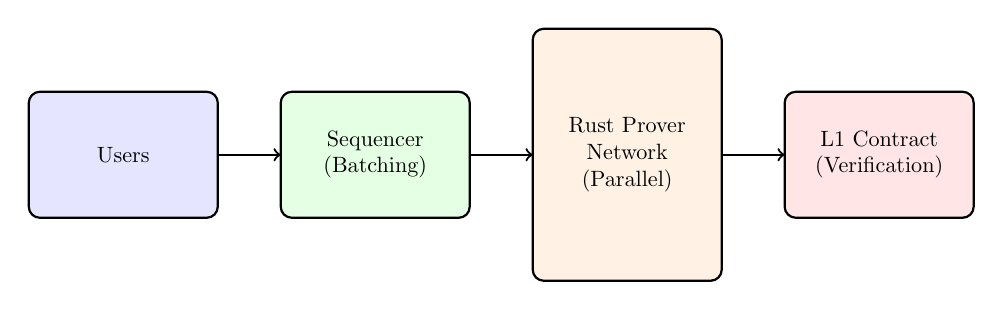
\begin{tikzpicture}[scale=0.8, transform shape]
        \draw[thick, rounded corners, fill=blue!10] (0,0) rectangle (3,2) node[pos=.5] {Users};
        \draw[thick, ->] (3,1) -- (4,1);
        \draw[thick, rounded corners, fill=green!10] (4,0) rectangle (7,2) node[pos=.5, align=center] {Sequencer \\ (Batching)};
        \draw[thick, ->] (7,1) -- (8,1);
        \draw[thick, rounded corners, fill=orange!10] (8,-1) rectangle (11,3) node[pos=.5, align=center] {Rust Prover \\ Network \\ (Parallel)};
        \draw[thick, ->] (11,1) -- (12,1);
        \draw[thick, rounded corners, fill=red!10] (12,0) rectangle (15,2) node[pos=.5, align=center] {L1 Contract \\ (Verification)};
    \end{tikzpicture}
    \captionof{figure}{System Architecture Diagram}
\end{center}

}

\headerbox{5. Implementation}{name=progress,column=1,below=arch,span=2,above=bottom}{

\begin{itemize}
    \item \textbf{Proving System:} Implemented using the \texttt{bellman} and \texttt{halo2} Rust crates.
    \item \textbf{Parallelization:} Utilized \texttt{rayon} for multi-threaded state tree updates and proof generation.
    \item \textbf{Testing:} Benchmarked on an AWS EC2 instance (32 cores, 64GB RAM) simulating a high-load sequencer environment.
\end{itemize}

\vspace{1em}
\begin{center}
\resizebox{0.9\textwidth}{!}{
\begin{tabular}{@{}lccc@{}}
\toprule
\textbf{Implementation} & \textbf{Batch Size} & \textbf{Proof Time (s)} & \textbf{TPS} \\ \midrule
Baseline (Sequential) & 1000 & 45.2 & 22.1 \\
Ours (4 Threads) & 1000 & 14.8 & 67.5 \\
Ours (16 Threads) & 1000 & 4.5 & 222.2 \\
Ours (32 Threads) & 1000 & 2.8 & \textbf{357.1} \\ \bottomrule
\end{tabular}
}
\captionof{table}{Throughput Comparison (Rust Implementation)}
\end{center}

}

% --- LAYER 3: THE BOTTOM ANCHORS --- 
\headerbox{6. Conclusions}{name=conclusion,column=0,below=background,span=1}{

\begin{itemize}
    \item \textbf{Scalability Achieved:} Parallel proof generation effectively shifts the bottleneck away from computation, maximizing ZK-Rollup throughput.
    \item \textbf{Efficiency:} The Rust-based prover network demonstrated near-linear scaling up to 16 cores.
    \item \textbf{Future Work:} Integrating hardware acceleration (GPUs/FPGAs) to further reduce proof latency and evaluating recursive SNARK limits.
\end{itemize}

}

\headerbox{7. References}{name=refs,column=0,below=conclusion,span=1,above=bottom}{ 
{\scriptsize 
\bibliographystyle{IEEEtranN}
\bibliography{custom}
}
}
\end{poster}
\end{document}
